\documentclass[12pt]{article}
\usepackage[MeX]{polski} % tak dodaje się Język Polski 
% kodowanie: latin2, utf8 lub cp1250
\usepackage[utf8]{inputenc} 
\usepackage{ulem}
\usepackage{graphicx}
\usepackage{wrapfig}
\usepackage{hyperref}
\usepackage{geometry}
\geometry{margin=31mm}

\begin{document}

\begin{titlepage}
\title{Moja pierwsza przykładowa praca w \LaTeX}
\author{Aleksandra Ostrowska}
\date{2024 rok}
\maketitle
\thispagestyle{empty}
\end{titlepage}

\begin{abstract}
To będzie bardzo interesujące, zapraszam do lektury.
\end{abstract}
\newpage

\part{Poezja}

\section{Dezyderata}
\paragraph{Max Ehrmann}
\paragraph{}
Przechodź spokojnie przez hałas i pośpiech, i pamiętaj, jaki spokój można znaleźć w ciszy.
\paragraph{}
O ile to możliwe, bez wyrzekania się siebie bądź na dobrej stopie ze wszystkimi.\\
Wypowiadaj swoją prawdę jasno i spokojnie, wysłuchaj innych, nawet tępych i nieświadomych, oni też mają swoja opowieść.\\
Unikaj głośnych i napastliwych - są udręką ducha.\\
\textit{Porównując się z innymi możesz stać się próżny i zgorzkniały, bowiem zawsze znajdziesz lepszych i gorszych od siebie.}
\paragraph{}
\underline{Niech twoje osiągnięcia zarówno jak plany będą dla Ciebie źródłem radości.}\\
Wykonaj swą pracę z sercem - jakakolwiek byłaby skromna, ją jedynie posiadasz
w zmiennych kolejach losu.\\
Bądź ostrożny w interesach, na świecie bowiem pełno oszustwa.\\
Niech Ci to jednak nie zasłoni prawdziwej cnoty; wielu ludzi dąży do wzniosłych ideałów
i wszędzie życie pełne jest heroizmu.
\paragraph{}
\textbf{Bądź sobą, zwłaszcza nie udawaj uczucia.}\\
Ani też nie podchodź \sout{cynicznie} do miłości, albowiem wobec oschłości i rozczarowań ona jest wieczna jak trawa.\\
Przyjmij spokojnie co Ci lata doradzają z wdziękiem wyrzekając się spraw młodości.
\paragraph{}
Rozwijaj siłę ducha, aby mogła cię osłonić w nagłym nieszczęściu.\\
Lecz nie dręcz się tworami wyobraźni. Wiele obaw rodzi się ze znużenia i samotności.\\
Obok zdrowej dyscypliny \textbf{bądź dla siebie łagodny.}\\
\textsc{Jesteś dzieckiem wszechświata nie mniej niż drzewa i gwiazdy, masz prawo być tutaj.}\\
I czy to jest dla ciebie jasne, czy nie - wszechświat bez wątpienia jest na dobrej drodze.
\paragraph{}
Tak więc żyj w zgodzie z Bogiem, czymkolwiek On ci się wydaje,\\
czymkolwiek się trudzisz i jakiekolwiek są twoje pragnienia, w zgiełkliwym pomieszaniu życia zachowaj spokój ze swą duszą.\\
Przy całej swej złudności, znoju i rozwianych marzeniach jest to piękny świat.\\
Bądź pogodny. \textbf{Dąż do szczęścia.}\cite{Dezyderata}

\section{Mój ulubiony wiersz}
\subsection{Dziewczyna}
\paragraph{Bolesław Leśmian}

\paragraph{}
Dwunastu braci, wierząc w sny, zbadało mur od marzeń strony,\\
A poza murem płakał głos, dziewczęcy głos zaprzepaszczony.\\
I pokochali głosu dźwięk i chętny domysł o Dziewczynie,\\
I zgadywali kształty ust po tym, jak śpiew od żalu ginie...\\
\paragraph{}

Mówili o niej: \textit{"Łka, więc jest!"} - I nic innego nie mówili,\\
I przeżegnali cały świat - i świat zadumał się w tej chwili...\\
Porwali młoty w twardą dłoń i jęli w mury tłuc z łoskotem!\\
\textbf{I nie wiedziała ślepa noc, kto jest człowiekiem, a kto młotem?}\\
\\
\textit{"O, prędzej skruszmy zimny głaz, nim śmierć Dziewczynę rdzą powlecze!" -}\\
Tak, waląc w mur, dwunasty brat do jedenastu innych rzecze.\\
Ale daremny był ich trud, daremny ramion sprzęg i usił!\\
\underline{Oddali ciała swe na strwon owemu snowi, co ich kusił!}\\
\\
Łamią się piersi, trzeszczy kość, próchnieją dłonie, twarze bledną...\\
I wszyscy w jednym zmarli dniu i noc wieczystą mieli jedną!\\
\paragraph{}

Lecz cienie zmarłych - \textit{Boże mój!} - nie wypuściły młotów z dłoni!\\
I tylko inny płynie czas - i tylko młot inaczej dzwoni...\\
I dzwoni w przód! I dzwoni wspak! I wzwyż za każdym grzmi nawrotem!\\
\textbf{I nie wiedziała ślepa noc, kto tu jest cieniem, a kto młotem?}\\
\\
\textit{"O, prędzej skruszmy zimny głaz, nim śmierć Dziewczynę rdzą powlecze!" -}\\
Tak, waląc w mur, dwunasty cień do jedenastu innych rzecze.\\
Lecz cieniom zbrakło nagle sił, a cień się mrokom nie opiera!\\
\underline{I powymarły jeszcze raz, bo nigdy dość się nie umiera...}\\
\\
I nigdy dość, i nigdy tak, jak pragnie tego ów, co kona!...\\
I znikła treść - i zginął ślad - i powieść o nich już skończona!\\
\paragraph{}

Lecz dzielne młoty - \textit{Boże mój} - mdłej nie poddały się żałobie!\\
I same przez się biły w mur, huczały śpiżem same w sobie!\\
Huczały w mrok, huczały w blask i ociekały ludzkim potem!\\
\textbf{I nie wiedziała ślepa noc, czym bywa młot, gdy nie jest młotem?}\\
\\
\textit{ "O, prędzej skruszmy zimny głaz, nim śmierć Dziewczynę rdzą powlecze!"} -\\
Tak, waląc w mur, dwunasty młot do jedenastu innych rzecze.\\
I runął mur, tysiącem ech wstrząsając wzgórza i doliny!\\
\underline{Lecz poza murem - nic i nic! Ni żywej duszy, ni Dziewczyny!}\\
\\
Niczyich oczu ani ust! I niczyjego w kwiatach losu!\\
Bo to był głos i tylko - głos, i nic nie było oprócz głosu!\\
\paragraph{}

Nic - tylko płacz i żal i mrok i niewiadomość i zatrata!\\
Takiż to świat! Niedobry świat! Czemuż innego nie ma świata?\\
\\
Wobec kłamliwych jawnie snów, wobec zmarniałych w nicość cudów,\\
Potężne młoty legły w rząd, na znak spełnionych godnie trudów.\\
I była zgroza nagłych cisz. I była próżnia w całym niebie!\\
\textsc{A ty z tej próżni czemu drwisz, kiedy ta próżnia nie drwi z ciebie?}\cite{Dziewczyna}
\paragraph{}

\newpage
\part{Matematyka \textless3}

\section{Dyskretna}
\subsection{Zadanie 1.1 Oblicz:}

\paragraph{a)}
$\sum_{i=1}^{n}i*2^i$ dla n = 0,1,2,3,4
\subparagraph{n=0}
$\sum_{i=1}^{0}i*2^i=0$ 
\subparagraph{n=1}
$\sum_{i=1}^{1}i*2^i=1*2=2$
\subparagraph{n=2}
$\sum_{i=1}^{2}i*2^i=2+2*2^2=2+8=10$
\subparagraph{n=3}
$\sum_{i=1}^{3}i*2^i=10+3*2^3=10+24=34$
\subparagraph{n=4}
$\sum_{i=1}^{4}i*2^i=34+4*2^4=34+64=98$

\paragraph{b)}
$\prod_{i=1}^{4}2i+1=(2+1)(4+1)(6+1)(8+1)=3*5*7*9=945$

\newpage
\part{Obrazki logiczne \textless3}
\section{Jak rozwiązywać obrazki logiczne?}
\subsection{Bierzesz obrazek logiczny\cite{Violet}:}
\includegraphics[scale=0.62]{violetEye}
\subsection{I go rozwiązujesz\cite{Ardna}:}

\includegraphics{violetEyeSolved}

\section{Where does violet eye color come from?}

\begin{wrapfigure}{r}{0.48\textwidth}
\centering
    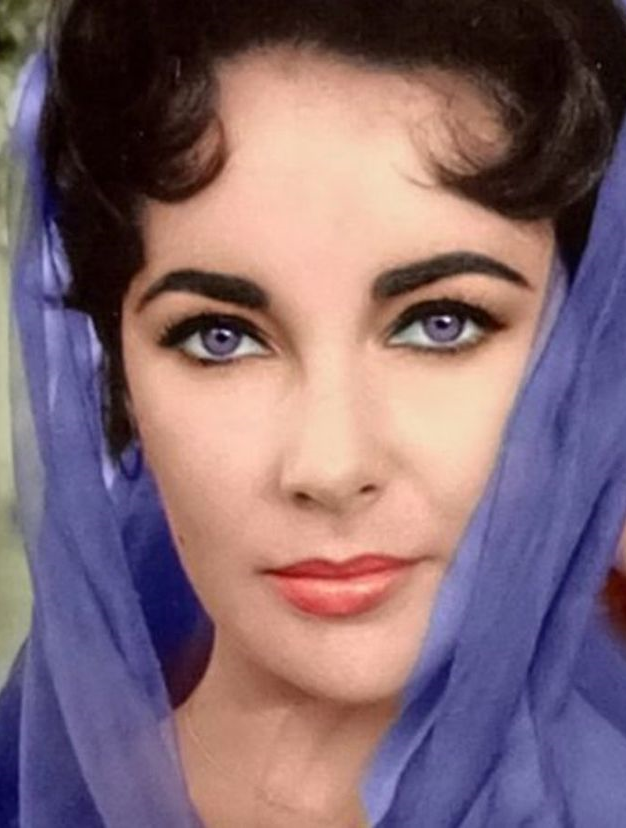
\includegraphics[width=0.435\textwidth]{Elizabeth}
    \caption{Elizabeth Taylor\cite{Elizabeth}}
\end{wrapfigure}

Eye color is puzzling by nature. Did you know blue eyes aren’t really blue?
\paragraph{}
The iris, the tinted part of your eye, contains melanin, the same substance that colors your skin and your hair. The people of Kenya, for instance, have far more melanin than their counterparts in Denmark. This helps explain why most Africans have dark skin and brown eyes, while many Europeans have light skin and blue eyes. 
\paragraph{}
The irises of blue-eyed people have no blue tint. Blue, it turns out, is in the eye of the beholder. You see it for the same reason the sky looks blue. Light waves get scattered in the earth’s atmosphere and in the irises of some humans. This makes the sky and some people’s eyes appear blue.  
\paragraph{}
Violet is an actual but rare eye color that is a form of blue eyes. It requires a very specific type of structure to the iris to produce the type of light scattering of melanin pigment to create the violet appearance.
\paragraph{}
Blue eyes are a recent arrival in human history. Some scientists believe all blue-eyed people trace their genetic heritage to a single mutation that happened perhaps 10,000 years ago.\cite{fiolet}

\section{Kolor oczu \textless3}

\begin{tabular}{l|l}
Kolor oczu 				& Populacja\\\hline
Brązowy 					& 55-79\%\\
Bursztynowy\slash piwny 	& 10\%\\
Zielony 					& 2\%\\
Szary i inne 				& mniej niż 1\%\\
\end{tabular}
\paragraph{}
There are four main eye colors—brown, blue, hazel, and green. Green was once considered the rarest eye color, but new classifications say another color may be even less common: gray.
\paragraph{}
Eye color is an inherited trait with multiple genes affecting the shade. Genes related to the production of pigments—melanin, eumelanin, and pheomelanin—dictate the color of your skin, hair, and eyes. A person's eye color reflects a unique combination and concentration of pigments in the iris.

\section{Gray: The Rarest Eye Color}
New classifications have determined that gray is its own standard color. With this change, gray now tops the list as the rarest eye color.
\paragraph{}
There's not much information on gray-colored eyes. In studies, gray and blue have historically been combined.
\paragraph{}
Gray eyes may contain just enough melanin in the front layer to dim the blue wavelengths of light that are reflected back by the tissue of the eye. Dark gray eyes have a bit more melanin in the front layer than pale gray eyes. 

\section{What Determines Eye Color?}
Eye color is influenced by the production of melanin, or pigments, in the iris—the colored part of your eye. More melanin means darker eyes; less means lighter eyes.
\paragraph{}
Different types of melanin determine the specific hue of the eyes. Eumelanin is a black-brown pigment responsible for darker eyes, hair, and skin. Pheomelanin is a yellow-red pigment that's behind green or amber eyes, red hair, and freckles.
\paragraph{}
People in countries farther away from the equator tend to have lighter-colored eyes and skin. Darker eyes and skin are common in warmer locales, closer to the equator. \cite{EColor}

\section{Bibliografia \textless3}
\begin{thebibliography}{3}
\bibitem{Dezyderata} Dezyderata \textless3 \href{https://www.fuw.edu.pl/~jziel/dezyderata.html}{Max Ehrmann}
\bibitem{Dziewczyna} Dziewczyna \href{https://literat.ug.edu.pl/lesman/dziewcz.htm}{Leśmian}
\bibitem{Violet} Violet Eye \href{https://www.griddlers.net/pl_PL/nonogram/-/g/65121}{by Ardna}
\bibitem{Ardna} Najlepszy autor obrazków logicznych w historii świata \href{https://www.griddlers.net/pl_PL/nonogram/-/g/p0/pp30/ta/sa/va/th0/i01/s0-100/c2-8/p1-100/d0-10000000000?_gpuzzles_WAR_puzzles_u=Ardna}{Invisible Pink Unicorn \textless3}
\bibitem{fiolet} Violet \href{https://www.allaboutvision.com/eye-care/eye-anatomy/violet-eyes/}{Eyes}
\bibitem{Elizabeth} Zdjęcie Pani Elizabeth Taylor: \href{https://pl.pinterest.com/pin/364017582374286320}{Pani Elizabeth Taylor}
\bibitem{EColor} Bardzo ciekawy artykuł po angielsku o kolorach oczu: \href{https://www.verywellhealth.com/what-is-the-rarest-eye-color-5087302}{Kolory Oczu oo}
\end{thebibliography}

\newpage
\tableofcontents
\end{document}